\begin{figure}[H]
    \centering
    \begin{subfigure}{\ResultSubFigureWidth \linewidth}
        \centering
        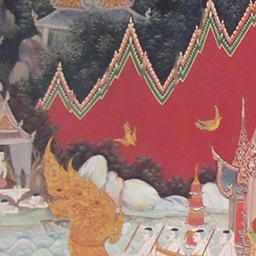
\includegraphics[width=\ResultSubFigurePadding \linewidth]{image/result_ex4/multisplitbergman_case01.png}
    \end{subfigure}
    \begin{subfigure}{\ResultSubFigureWidth \linewidth}
        \centering
        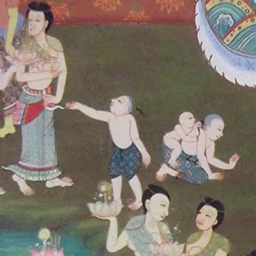
\includegraphics[width=\ResultSubFigurePadding \linewidth]{image/result_ex4/multisplitbergman_case02.png}
    \end{subfigure}
    \begin{subfigure}{\ResultSubFigureWidth \linewidth}
        \centering
        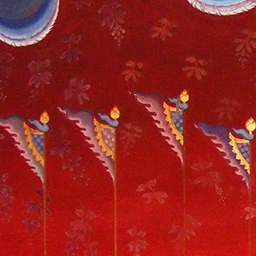
\includegraphics[width=\ResultSubFigurePadding \linewidth]{image/result_ex4/multisplitbergman_case03.png}			
    \end{subfigure}
    \begin{subfigure}{\ResultSubFigureWidth \linewidth}
        \centering
        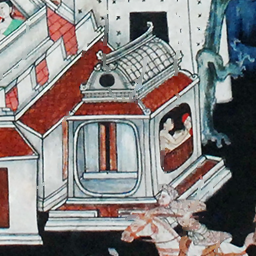
\includegraphics[width=\ResultSubFigurePadding \linewidth]{image/result_ex4/multisplitbergman_case04.png}			
    \end{subfigure}
    \begin{subfigure}{\ResultSubFigureWidth \linewidth}
        \centering
        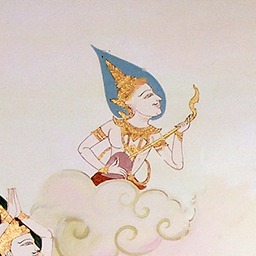
\includegraphics[width=\ResultSubFigurePadding\linewidth]{image/result_ex4/multisplitbergman_case05.png}			
    \end{subfigure}
    \caption{ผลการซ่อมแซมภาพโดยวิธีการเชิงตัวเลขที่พัฒนาขึ้น}
\end{figure}